\documentclass[11pt]{article}

\usepackage[portuguese]{babel}
\usepackage[utf8]{inputenc}
\usepackage{amsmath}
\usepackage{graphicx}
\usepackage{float}
\usepackage{subfig}
\usepackage{fixltx2e}
\usepackage[bottom]{footmisc}
\usepackage{color}
\usepackage[usenames,dvipsnames]{xcolor}
\usepackage[font=footnotesize]{caption}
\numberwithin{equation}{section}

\linespread{1.3}
\usepackage{indentfirst}
\usepackage[top=2cm, bottom=2cm, right=2.5cm, left=2.5cm]{geometry}
\addto\captionsportuguese{\renewcommand{\contentsname}{Índice}}

\begin{document}

\begin{titlepage}
\begin{center}

\hfill \break
\hfill \break


\includegraphics[width=0.3\textwidth]{./logo}~\\[1cm]

\textsc{\LARGE Instituto Superior Técnico}\\[0.25cm]
\textsc{\Large Mestrado Integrado em Engenharia Electrotécnica e de Computadores}\\[1.8cm]
\textsc{\huge Microelectrónica}\\[0.25cm]

{\huge \bfseries Espelho de Corrente \\[1cm]}

\begin{tabular}{ l l }
João Duarte Turras Guilherme & \hspace{2mm} n.º 70042 \\
Ana Cláudia Sarmento Ramos Marques & \hspace{2mm} n.º 72725 \\
Maria Margarida Dias dos Reis & \hspace{2mm} n.º 73099
\end{tabular}

\vfill

{\large Lisboa, 30 de Janeiro de 2014} 

\end{center}
\end{titlepage}

\pagenumbering{gobble}
\clearpage

\tableofcontents
\pagebreak

\clearpage
\pagenumbering{arabic}

\section{Introdução}

As fontes de corrente são um componente essencial da electrónica e assim, é importante perceber como são fabricadas. Tipicamente, as fontes de correntes dentro de blocos são implementadas com recurso a espelhos de corrente. O espelho de corrente é o circuito que se projecta com o intuito de copiar a corrente que passa por um dispositivo activo através do controlo da corrente noutro dispositivo activo do circuito, mantendo a corrente de saída constante, independentemente da carga. Assim, o espelho de corrente é utilizado para fornecer correntes de \textit{bias} (correntes de polarização) e cargas activas a circuitos. 

Com este trabalho de laboratório pretende-se explorar o funcionamento do espelho de corrente básico e do espelho de corrente \textit{cascode}.

\pagebreak

\section{Espelho de corrente básico}
\subsection{Tensão de \textit{Overdrive}}

Pretende-se projectar um espelho de corrente básico da seguinte forma:

\begin{figure}[h]
	\centering
	\includegraphics[keepaspectratio=true, scale=0.35]{teoricas/imagem1}
	\vspace{-0.8em}
	\caption{Espelho de corrente básico.}
	\vspace{-0.8em}
\end{figure} 

O transístor M\textsubscript{1} deve ter uma tensão de \textit{overdrive} ($V_{OD}$) de 0.2V com uma corrente $I_{0}$ de 10$\mu$A. O transístor M\textsubscript{2} deve ter uma corrente $I_{1}$ igual a $I_{0}$, logo os dois transístores devem ter as mesmas dimensões.

Sabe-se que a corrente num transístor MOS é dada por:

\vspace{-3mm}
\begin{equation}
I_{D} = \frac{1}{2}\mu_{n}C_{ox}\times \Big(\frac{W}{L}\Big) \times(V_{GS}-V_{TH})^2 = k\times \Big(\frac{W}{L}\Big) \times V_{OD}^2
\label{eq:corrente}
\end{equation}

\vspace{1mm}
e através da corrente é possível determinar as dimensões do transístor. 

O funcionamento deste espelho de corrente, ignorando o efeito de modulação do comprimento do canal, é dado por:

\begin{equation}
\begin{cases}I_{bias10u} = k\times \Big(\frac{W}{L}\Big)_{1} \times(V_{GS}-V_{TH})^2 \\ I_{out} = k\times \Big(\frac{W}{L}\Big)_{2} \times(V_{GS}-V_{TH})^2 \vspace{2mm} \\ I_{out} = \frac{({W}/{L})_{2}}{({W}/{L})_{1}} \times I_{bias10u} \end{cases}
\end{equation}

\vspace{2mm}
Como se pode ver, o rácio entre a corrente de referência ($I_{bias10u}$) e a corrente de saída ($I_{out}$) é dado pelo rácio das dimensões dos transístores que constituem o espelho de corrente.

Neste caso, para M\textsubscript{1} é conhecido o valor da corrente, da tensão de \textit{overdrive} e o valor de $k$ (factor de ganho) pode ser obtido consultando os \textit{process parameters}\footnote{Página 11 - valor de KPN.} da tecnologia em uso (CMOS C35). Assim, verifica-se que o valor de $k$ para um transístor NMOS é 170. Recorrendo agora à equação~\ref{eq:corrente} pode-se obter as dimensões de M\textsubscript{1}.

\vspace{-3mm}
\begin{equation}
I_{D_{1}} = k\times \Big(\frac{W}{L}\Big)_{1} \times V_{OD}^2 \leftrightarrow \Big(\frac{W}{L}\Big)_{1} = \frac{I_{D_{1}}}{kV_{OD}^2} \leftrightarrow \Big(\frac{W}{L}\Big)_{1} = 1.47.
\end{equation}

\vspace{1mm}
Sabendo que se utiliza o valor mínimo de $L$ que a tecnologia permite, ou seja, 0.35$\mu$m então o valor de $W$ é de 0.5147$\mu$m. Essas são as dimensões dos transístores M\textsubscript{1} e M\textsubscript{2}.

No esquema do espelho de corrente básico os transístores foram instanciados com um comprimento $Lpar$ e uma largura $Wpar$. Projecta-se o esquema do espelho de corrente e também o símbolo correspondente, que deve ser intuitivo sobre qual a função desempenhada pela célula.

\begin{figure}[H]
	\centering
	\subfloat[]{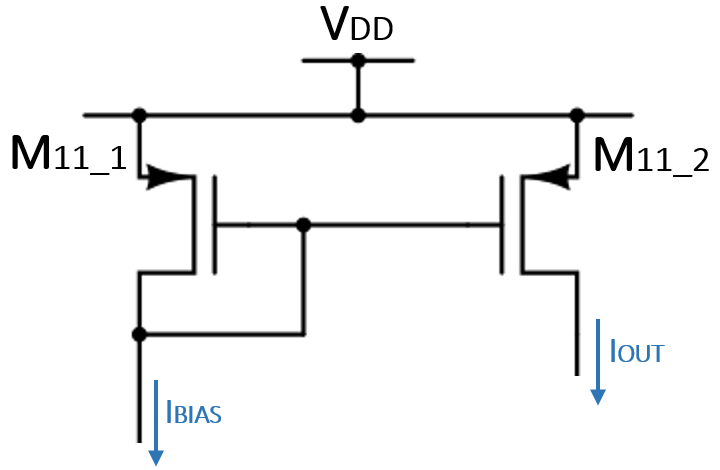
\includegraphics[keepaspectratio=true, scale=0.40]{esquemas/cmirror}}
	\hspace{2mm}
	\subfloat[]{\includegraphics[keepaspectratio=true, scale=0.386]{esquemas/cmirror_sym}}
	\vspace{-0.8em}
	\caption{Esquema do espelho de corrente básico (a) e correspondente símbolo (b).}
    \vspace{-0.8em}
\end{figure}

\subsection{Efeito de modulação do comprimento do canal}

Cria-se também um esquema de \textit{testbench} que fornece a corrente de \textit{bias} e efectua um varrimento da tensão $V_{DS}$ de M\textsubscript{2}, o que pretende demonstrar que a fonte de corrente de 10$\mu$A foi implementada como esperado.

Na Figura~\ref{fig:simul1} está a característica do espelho de corrente básico que foi projectado para dois valores de $L$, o mínimo de 0.35$\mu$m e dez vezes o valor mínimo.

\begin{figure}[H]
	\centering
	\includegraphics[keepaspectratio=true, scale=0.40]{simuls/simul1}
	\vspace{-0.8em}
	\caption{Característica do espelho de corrente básico para dois valores diferentes de $L$.}
	\vspace{-0.8em}
	\label{fig:simul1}
\end{figure} 

Como se pode ver, quando se utiliza o valor mínimo de $L$ a característica sofre dispersão à medida que $V_{DS}$ aumenta. Quando se utiliza um $L$ que é dez vezes maior que o mínimo, a característica tem uma forma melhor (mais próxima da ideal), sem sofrer de dispersão. Esta conclusão sugere a ocorrência de um fenómeno de segunda-ordem, que será abordado mais à frente. No entanto, apesar destas conclusões, um valor de 3.5$\mu$m é muito elevado para aquilo que a tecnologia actual permite. 

Outra simulação que é interessante fazer permite verificar qual é a característica do espelho de corrente básico quando se varia o comprimento, mantendo fixo o valor da largura. Assim, optou-se por um $W$ de 2$\mu$m e fez-se variar o valor de $L$. O resultado gerado é apresentado de seguida.

\begin{figure}[H]
	\centering
	\subfloat[]{\includegraphics[keepaspectratio=true, scale=0.50]{simuls/simul1_difsat}}
	\linebreak
	\subfloat[]{\includegraphics[keepaspectratio=true, scale=0.50]{simuls/simul1_difsat_zoom}}
	\vspace{-0.8em}
	\caption{Simulação efectuada para o espelho de corrente básico com um valor de $W$ fixo e $L$ variável (a) e \textit{zoom} dessa simulação na zona de entrada na saturação dos transístores (b).}
	\vspace{-0.8em}
\end{figure}

Para se analisar as figuras anteriores é necessário explorar melhor o conceito de tensão de \textit{overdrive}. Matematicamente, esta tensão pode ser expressa por:

\vspace{-3mm}
\begin{equation}
V_{OD} = V_{GS}-V_{TH}
\end{equation}

\vspace{1mm}
e é uma medida de quando o transístor entra na saturação, ou seja, de quão longe está da zona de corte.

Pela Figura 4(b), percebe-se que para diferentes valores de $L$ a entrada na saturação varia também (as várias características têm diferentes declives), ou seja, a tensão de \textit{overdrive} varia de caso para caso. Quando a tensão de \textit{overdrive} é menor, o transístor entra na saturação mais cedo e quando é maior, o transístor entra na saturação mais tarde. Para valores de $L$ maiores a entrada na saturação ocorre mais tarde, ou seja, a tensão de \textit{overdrive} é maior, caso da curva que tem $L = 6\mu$m. A curva com $L = 0.35\mu$m é aquela em que a característica apresenta maior dispersão, como se viu anteriormente, e a entrada na saturação ocorre mais cedo, ou seja, a tensão de \textit{overdrive} é menor.

Pode-se também simular o comportamento do circuito para o caso em que se fixa o valor de $L$ a 1$\mu$m, fazendo-se variar o valor de $W$.

\begin{figure}[H]
	\centering
	\includegraphics[keepaspectratio=true, scale=0.50]{simuls/ovL1Wmuda}
	\vspace{-0.8em}
	\caption{Característica do espelho de corrente básico para transístores com $L$ fixo de 1$\mu$m e $W$ de 0.5$\mu$m, 2$\mu$m e 4$\mu$m.}
	\vspace{-0.8em}
\end{figure} 

Para valores de $W$ maiores a entrada na saturação ocorre mais cedo, a tensão de \textit{overdrive} é portanto menor. Conclui-se então, que quanto menor for o $L$ mas maior for o $W$ a tensão de \textit{overdrive} é menor, existindo um compromisso na variação deste dois parâmetros.

Assim, conclui-se que, para que a tensão de \textit{overdrive} seja a mesma, quando se varia o valor do comprimento, é necessário que o valor de $W$ esteja dependente de $L$, ou seja, $Wpar = Lpar\times1.47$. Com esta dependência estabelecida, voltou-se a simular o circuito fazendo variar o comprimento. O resultado obtido é apresentado de seguida.

\begin{figure}[H]
	\centering
	\subfloat[]{\includegraphics[keepaspectratio=true, scale=0.50]{simuls/simul1_satigual}}
\end{figure}

\begin{figure}[H]
	\centering
	\subfloat[]{\includegraphics[keepaspectratio=true, scale=0.50]{simuls/simul1_satigual_zoom}}
	\vspace{-0.8em}
	\caption{Simulação efectuada para o espelho de corrente básico com um valor de $W$ variável de acordo com o valor de $L$ (a) e \textit{zoom} dessa simulação na zona de entrada na saturação dos transístores (b).}
	\vspace{-0.8em}
\end{figure}

Como se pode ver, para o caso em que $W$ varia de acordo com $L$, a entrada na saturação ocorre na mesma altura (as várias características têm o mesmo declive), logo a tensão de \textit{overdrive} é a mesma. No entanto, conclui-se que para valores menores de $L$ a característica apresenta distorção à medida que $V_{DS}$ aumenta. Assim, fala-se num efeito de segunda-ordem: efeito de modulação do comprimento do canal, que pode melhor ser entendido olhando para a equação

\vspace{-3mm}
\begin{equation}
I_{D} \approx \frac{1}{2}\mu_{n}C_{ox}\times \Big(\frac{W}{L}\Big) \times(V_{GS}-V_{TH})^2 (1+\lambda V_{DS}).
\end{equation}

\vspace{1mm}
Idealmente quer-se que a corrente $I_{D}$ seja apenas dependente de $V_{GS}$, no entanto, apresenta de facto também uma dependência com $V_{DS}$, de acordo com o coeficiente de modulação do comprimento do canal, $\lambda$. 

Assim, a relação entre as correntes do espelho de corrente passa a ser dada por:

\vspace{-3mm}
\begin{equation}
I_{out} = \frac{({W}/{L})_{2}}{({W}/{L})_{1}} \times \frac{1+\lambda V_{DS_{2}}}{1+\lambda V_{DS_{1}}} \times I_{bias10u}
\label{eq:iout}
\end{equation}

\vspace{1mm}
Como se verifica a existência deste efeito de segunda-ordem, a característica do espelho de corrente tem um declive diferente de 0 na zona de saturação, tal como se verifica na Figura 3, na Figura 4(a) e na Figura 6(a). 

Assim, quando se verifica o efeito de modulação do comprimento do canal, a fonte de corrente que se encontra ligada ao circuito e que lhe fornece a corrente de polarização é de facto da seguinte forma.

\begin{figure}[H]
	\centering
	\includegraphics[keepaspectratio=true, scale=0.30]{teoricas/imagem3}
	\vspace{-0.5em}
	\caption{Comportamento equivalente da fonte de corrente quando se sofre de efeito de modulação do comprimento do canal.}
	\vspace{-0.8em}
\end{figure} 

A resistência que existe em paralelo com a fonte de corrente é de valor $1/\lambda$. Este parâmetro $\lambda$ representa a variação relativa no comprimento do canal para um dado incremento de $V_{DS}$ e, como tal, para canais mais compridos, $\lambda$ será menor e o efeito de modulação do comprimento do canal sente-se menos. Isto é comprovado pela Figura 6(a), pois a curva correspondente ao maior $L$ de todos ($Lpar = 6\mu$m) é a que apresenta um declive mais próximo de 0 na zona de saturação, ou seja, é a mais próxima da característica ideal. Assim, quanto maior for o comprimento do canal, menor será o valor de $\lambda$ e a resistência estará mais próxima de $\infty$, que é o valor ideal. 

Como \textit{rule of thumb}, para se evitar o efeito de modulação do comprimento do canal, opta-se por um valor de $L$ maior ou igual a 1$\mu$m.

\subsection{\textit{Mismatch}}

Na realidade, os circuitos nunca são perfeitamente simétricos - os dois lados não exibem propriedades idênticas pois os componentes nunca são ideais. Assim, para o caso do espelho de corrente básico, os dois transístores M\textsubscript{1} e M\textsubscript{2} nunca vão ser iguais, o que leva a erros de \textit{mismatch} entre os dois componentes.

Pretende-se calcular o erro relativo do espelho de corrente. Negligenciando o efeito de modulação do comprimento do canal, consegue-se determinar o \textit{mismatch} total entre $I_{D_{1}}$ e $I_{D_{2}}$ através do cálculo da derivada total.

\vspace{-3mm}
\begin{equation}
\Delta y = \frac{\partial f}{\partial x_{1}}\Delta x_{1} + \frac{\partial f}{\partial x_{2}}\Delta x_{2} + \cdots.
\label{eq:mismatch}
\end{equation}

\vspace{1mm}
Na equação~\ref{eq:mismatch}, percebe-se que o cálculo da derivada total é dado pela soma de cada componente de \textit{mismatch} ($\Delta x_{j}$) multiplicada pela respectiva sensibilidade (${\partial f}/{\partial x_{j}}$).

Segundo a equação~\ref{eq:corrente} tem-se:

\vspace{-3mm}
\begin{equation}
\Delta I_{D} = \frac{\partial I_{D}}{\partial ({W}/{L})}\Delta \Big(\frac{W}{L}\Big) + \frac{\partial I_{D}}{\partial (V_{GS}-V_{TH})}\Delta (V_{GS}-V_{TH})
\end{equation}

\vspace{1mm}
onde os erros relativos a $\mu_{n}$$C_{ox}$ são desprezados. Assim,

\vspace{-3mm}
\begin{equation}
\Delta I_{D} = \frac{1}{2}\mu_{n}C_{ox}(V_{GS}-V_{TH})^2 \Delta \Big(\frac{W}{L}\Big) - \mu_{n}C_{ox}\Big(\frac{W}{L}\Big)(V_{GS}-V_{TH})\Delta V_{TH}.
\end{equation}

\vspace{1mm}
Normalizando o erro da corrente em relação ao seu valor médio obtém-se

\vspace{-3mm}
\begin{equation}
\frac{\Delta I_{D}}{I_{D}} = \frac{\Delta({W}/{L})}{{W}/{L}} - 2 \frac{\Delta V_{TH}}{V_{GS}-V_{TH}}.
\end{equation}

\vspace{1mm}
Portanto, para minimizar o erro da corrente deve-se maximizar a tensão de \textit{overdrive}, $V_{OD}$, que toma um valor típico de $200m$V.

Quando se projectou o espelho de corrente, ambos os transístores ficaram com as mesmas dimensões: comprimento $Lpar$ e largura $Wpar = Lpar \times 1.47$. Assim, assume-se que não há erros relativos ao dimensionamento dos transístores e como tal $\Delta({W}/{L}) = 0$.

A equação 2.10 fica então simplificada a:

\vspace{-3mm}
\begin{equation}
\frac{\Delta I_{D}}{I_{D}} = - 2 \frac{\Delta V_{TH}}{V_{GS}-V_{TH}} = -2 \frac{\Delta V_{TH}}{V_{OD}},
\end{equation}

\vspace{1mm}
sendo que para determinar o \textit{mismatch} entre as correntes nos dois transístores é necessário determinar $\Delta V_{TH}$. De notar que a tensão de \textit{threshold} depende sobretudo da espessura do óxido sob a \textit{gate} e da concentração de portadores no canal. A variação na tensão de \textit{threshold} é calculada da seguinte maneira:

\vspace{-3mm}
\begin{equation}
\Delta V_{TH} = \frac{A_{V_{T}}}{\sqrt{W \times L}},
\end{equation}

\vspace{1mm}
sendo $A_{V_{T}}$ um parâmetro da tecnologia, correspondente à constante de \textit{mismatch} SOMETHING e como tal a variação na tensão de \textit{threshold} é calculada da seguinte forma:

\vspace{-3mm}
\begin{equation}
\Delta V_{TH} = \frac{A_{V_{T}}}{\sqrt{Wpar \times Lpar}} = \frac{VALOR}{\sqrt{Lpar \times 1.47 \times Lpar}} = \frac{VALOR}{\sqrt{Lpar ^2\times 1.47}}.
\end{equation}

\vspace{1mm}
Para o caso de um comprimento de 1$\mu$m (valor que minimiza o efeito de modulação do comprimento do canal) a variação na tensão de \textit{threshold} toma o seguinte valor:

\vspace{-3mm}
\begin{equation}
\Delta V_{TH} = \frac{VALOR}{\sqrt{Lpar ^2\times 1.47}} = \frac{VALOR}{\sqrt{(10^{-6})^2\times 1.47}}
\end{equation}

\vspace{1mm}
E com este valor é possível determinar o \textit{mismatch} entre as correntes do espelho de corrente:

\vspace{-3mm}
\begin{equation}
\frac{\Delta I_{D}}{I_{D}} = - 2 \frac{\Delta V_{TH}}{V_{GS}-V_{TH}} = - 2 \frac{\Delta V_{TH}}{V_{OD}} = - 2 \times \frac{VALOR ANTES}{0.2}
\end{equation}

\vspace{1mm}
ACABAR MISMATCH

\subsection{Simulação por \textit{corners}}

Pretende-se agora efectuar uma simulação por \textit{corners} do espelho de corrente básico. Inicialmente, foram efectuadas três simulações para a característica $I_{D}/V_{DS}$, cada uma com o valor mínimo de $L$ (0.35$\mu$m) e um valor de $W$ diferente: 0.5$\mu$m, 2$\mu$m e 4$\mu$m. Com esta experiência pretende-se entender qual o efeito da tensão de \textit{overdrive} no correcto funcionamento do circuito.

\begin{figure}[H]
	\centering
	\hspace*{-0.8cm}
	\subfloat[]{\includegraphics[keepaspectratio=true, scale=0.28]{simuls/corners_L035_W05}}
	\hspace*{0.5cm}
	\subfloat[]{\includegraphics[keepaspectratio=true, scale=0.28]{simuls/corners_L035_W05_zoom}}
	\vspace{-0.8em}
	\caption{Simulação por \textit{corners} do espelho de corrente básico com $L = 0.35\mu$m e $W = 0.5\mu$m (a) e \textit{zoom} dessa simulação na zona de entrada na saturação dos transístores (b).}
	\vspace{-0.8em}
\end{figure}

\begin{figure}[H]
	\centering
	\hspace*{-0.8cm}
	\subfloat[]{\includegraphics[keepaspectratio=true, scale=0.28]{simuls/corners_L035_W2}}
	\hspace*{0.5cm}
	\subfloat[]{\includegraphics[keepaspectratio=true, scale=0.28]{simuls/corners_L035_W2_zoom}}
	\vspace{-0.8em}
	\caption{Simulação por \textit{corners} do espelho de corrente básico com $L = 0.35\mu$m e $W = 2\mu$m (a) e \textit{zoom} dessa simulação na zona de entrada na saturação dos transístores (b).}
	\vspace{-0.8em}
\end{figure}

\begin{figure}[H]
	\centering
	\hspace*{-0.8cm}
	\subfloat[]{\includegraphics[keepaspectratio=true, scale=0.28]{simuls/corners_L035_W4}}
	\hspace*{0.5cm}
	\subfloat[]{\includegraphics[keepaspectratio=true, scale=0.28]{simuls/corners_L035_W4_zoom}}
	\vspace{-0.8em}
	\caption{Simulação por \textit{corners} do espelho de corrente básico com $L = 0.35\mu$m e $W = 4\mu$m (a) e \textit{zoom} dessa simulação na zona de entrada na saturação dos transístores (b).}
	\vspace{-0.8em}
\end{figure}

Primeiramente, verifica-se que quanto menor for o valor da largura, maior será a tensão de \textit{overdrive}, ou seja, os transístores entram mais tarde na saturação. Das três simulações percebe-se que para o maior $W$ (4$\mu$m), a tensão de \textit{overdrive} é a menor, pois aqui a característica está mais ``encostada'' à esquerda.

É também nessa simulação que se verifica maior dispersão nas várias características - para um mesmo valor de $V_{DS}$, é aqui que a corrente $I_{D}$ toma valores mais elevados e, consequentemente, mais afastados do valor pretendido de 10$\mu$A. Assim se percebe como, quanto menor for a tensão de \textit{overdrive}, mais sensível se fica à tensão de \textit{threshold}, $V_{TH}$.

Explica-se então que a \textit{rule of thumb} seja escolher para $V_{OD}$ um valor de 0.2V - menos do que isso e fica-se demasiado sensível a $V_{TH}$ e mais do que isso e fica-se com pouca margem de saturação, que é uma medida do quão dentro da saturação se está, sendo calculado por $V_{DS} - V_{OD}$.

Relativamente ao \textit{zoom} que foi efectuado na zona da característica de entrada na saturação dos transístores do espelho de corrente, percebe-se como para um dado valor de tensão, por exemplo $V_{DS} = 200m$V, para o menor valor de $W$ a corrente toma valores menores e consequentemente a tensão de \textit{overdrive} será maior.

Outra simulação feita por \textit{corners} foi para uma tensão de \textit{overdrive} constante, optando-se por um comprimento $Lpar = 3.5\mu$m e uma largura igual a $Wpar = Lpar\times1.47$.

\begin{figure}[h]
	\centering
	\includegraphics[keepaspectratio=true, scale=0.50]{simuls/corners_good}
	\vspace{-0.8em}
	\caption{Simulação por \textit{corners} com um valor de $W$ variável de acordo com o valor de $L = 3.5\mu$m.}
	\vspace{-0.8em}
\end{figure} 

Verifica-se o correcto comportamento do circuito para situações extremas de funcionamento, como por exemplo de temperatura.

De notar que as várias características têm todas declive próximo de 0 na zona da saturação porque se utiliza um $L$ que é dez vezes maior que o mínimo da tecnologia.

\pagebreak

\section{Espelho de corrente \textit{cascode}}

Como se viu na Secção 2, o espelho de corrente básico tem uma corrente de saída que apresenta uma dependência com a tensão $V_{DS}$ do transístor de saída. Para reduzir essa dependência, pode-se usar transístores com um comprimento de canal superior a 1$\mu$m. Mais ainda, projectar um circuito com tensões de \textit{overdrive} superiores a 0.2V também limita esta dependência de $V_{DS}$ quando se faz uma análise por \textit{corners}.

Pretende-se agora explorar as vantagens de adicionar transístores \textit{cascode} ao espelho de corrente. Mais ainda, faz-se o \textit{design} do \textit{layout} do espelho de corrente \textit{cascode low voltage}.

\subsection{Espelho de corrente \textit{cascode} básico}

Pretende-se projectar um espelho de corrente \textit{cascode} básico da seguinte forma:

\begin{figure}[h]
	\centering
	\includegraphics[keepaspectratio=true, scale=0.33]{teoricas/imagem2}
	\vspace{-0.8em}
	\caption{Espelho de corrente \textit{cascode} básico.}
	\vspace{-0.8em}
\end{figure} 

No esquema elaborado todos os transístores têm as mesmas dimensões: comprimento $Lpar$ e uma largura $Wpar$.

\begin{figure}[H]
	\centering
	\subfloat[]{\includegraphics[keepaspectratio=true, scale=0.40]{esquemas/cmirror_casc}}
	\hspace{2mm}
	\subfloat[]{\includegraphics[keepaspectratio=true, scale=0.393]{esquemas/cmirror_casc_sym}}
	\vspace{-0.8em}
	\caption{Esquema do espelho de corrente \textit{cascode} básico (a) e correspondente símbolo (b).}
	\vspace{-0.8em}
\end{figure}

De seguida, aplicou-se a mesma fonte de tensão no espelho de corrente básico e no \textit{cascode}, comparando as suas correntes e tensões internas para um \textit{sweep} de tensão DC.

\begin{figure}[h]
	\centering
	\includegraphics[keepaspectratio=true, scale=0.53]{simuls/simul2_comp1}
	\vspace{-0.8em}
	\caption{Comparação da característica do espelho de corrente básico e do espelho de corrente \textit{cascode} básico.}
	\vspace{-0.8em}
\end{figure} 

Como se pode observar, o espelho de corrente \textit{cascode} é melhor que o espelho de corrente básico pois a corrente satura exactamente a 10$\mu$A, enquanto que no último a corrente ultrapassa este valor.

Na equação~\ref{eq:iout} verifica-se como a relação entre as correntes do espelho de corrente básico é afectada pelo efeito de modulação do comprimento do canal, problema que se resolve com um espelho de corrente \textit{cascode}.

Assim, o princípio de funcionamento é: os transístores M\textsubscript{1} e M\textsubscript{2} são usados para formar um espelho de corrente básico e os transístores M\textsubscript{0} e M\textsubscript{3} que formam o andar \textit{casc}ode são usados para que $V_{DS_{1}} = V_{DS_{2}}$. Desta maneira, o espelho de corrente formado por M\textsubscript{1} e M\textsubscript{2} para além de ter $V_{GS}$ iguais, tem também $V_{DS}$ iguais, o que forma um bom espelho de corrente - uma fonte de corrente praticamente ideal, como se pode observar na Figura 14 na zona em que os transístores estão na saturação. Aqui a corrente toma um valor de 10$\mu$A, não se fazendo sentir o efeito de modulação do comprimento do canal, como pretendido com a aplicação desta topologia.

A tensão no ponto $Y$ depende do comportamento do transístor M\textsubscript{3} que por sua vez está dependente da corrente. Analisando o circuito da Figura 12 conclui-se que $V_{GS_{0}} + V_{X} = V_{GS_{3}} + V_{Y}$. Se $V_{GS_{0}} = V_{GS_{3}}$ então $V_{X} = V_{Y}$, como pretendido. A igualdade entre as tensões $V_{GS}$ dos transístores M\textsubscript{0} e M\textsubscript{3} é garantida se $({W}/{L})_{3}/({W}/{L})_{0} = ({W}/{L})_{2}/({W}/{L})_{1}$, ou seja, se a corrente $I_{D_{0}} = I_{D_{1}}$ e a corrente $I_{D_{3}} = I_{D_{2}}$. Se $V_{X} = V_{Y}$, então os transístores do espelho de corrente têm $V_{GS}$ iguais, bem como $V_{DS}$ iguais, como era o objectivo.

Para verificar o funcionamento descrito anteriormente efectuou-se uma simulação do circuito, que pode ser vista na Figura 15.

\pagebreak

\begin{figure}[h]
	\centering
	\includegraphics[keepaspectratio=true, scale=0.45]{simuls/parte2_tensoes1}
	\vspace{-0.8em}
	\caption{Característica do espelho de corrente \textit{cascode} básico e tensões internas deste.}
	\vspace{-0.8em}
\end{figure} 

Como se pode ver, $V_{GS_1} = V_{GS_2}$ e a tensão $V_{DS_1}$ é constante e igual a $V_{DS_2}$ na zona de saturação, ou seja, verifica-se aqui o comportamento do espelho de corrente constituído pelos transístores M\textsubscript{1} e M\textsubscript{2} com tensões $V_{GS}$ iguais bem como tensões $V_{DS}$ iguais. 

No entanto, e como se verificou na Figura 14 e na Figura 15, apesar do espelho de corrente \textit{cascode} garantir que a corrente na zona de saturação está com o valor desejado de 10$\mu$A existe um compromisso que se relaciona com a margem de saturação. Como se pode verificar pela simulação, para o espelho de corrente \textit{cascode} a tensão de \textit{overdrive} é maior e consequentemente a margem de saturação ($V_{DS} - V_{OD}$) será menor comparativamente ao espelho de corrente básico, o que é um \textit{side effect} indesejado.

\subsection{Espelho de corrente \textit{cascode low voltage} e margem de saturação}

Para poder eliminar o \textit{trade-off} que há entre a exactidão do espelho de corrente \textit{cascode} e o consumo de tensão de \textit{headroom} recorre-se a uma topologia do espelho de corrente \textit{cascode low voltage}, que tem a seguinte forma:

\begin{figure}[H]
	\centering
	\includegraphics[keepaspectratio=true, scale=0.35]{teoricas/imagem4}
	\vspace{-0.8em}
	\caption{Espelho de corrente \textit{cascode low voltage}.}
	\vspace{-0.8em}
\end{figure}

O esquema criado para este circuito e o corresponde símbolo apresentam-se de seguida.

\begin{figure}[H]
	\centering
	\subfloat[]{\includegraphics[keepaspectratio=true, scale=0.41]{esquemas/cmirror_casc_vcasn}}
	\hspace{2mm}
	\subfloat[]{\includegraphics[keepaspectratio=true, scale=0.38]{esquemas/cmirror_casc_vcasn_sym}}
	\vspace{-0.8em}
	\caption{Esquema do espelho de corrente \textit{cascode low voltage} (a) e correspondente símbolo (b).}
	\vspace{-0.8em}
\end{figure}

De modo a construir o circuito \textit{low voltage} adiciona-se uma tensão de entrada $vcasn$ nas \textit{gates} dos transístores M\textsubscript{0} e  M\textsubscript{3}. Quer-se definir esta tensão de forma a que a margem de saturação do transístor M\textsubscript{1} seja 0V e que a tensão de \textit{overdrive} do transístor M\textsubscript{0} seja 0.2V. De relembrar que a margem de saturação define-se como a diferença entre $V_{DS_{1}}$ e $V_{OD_{1}}$.

Para que os transístores possam saturar para o menor valor de $V_{DS}$ possível, ou seja, para que haja um mínimo de consumo de tensão de \textit{headroom}, vem que $V_{X} = V_{GS_{1}} - V_{TH_{1}}$ e como tal $vcasn$ deve ser igual (ou ligeiramente maior) que $V_{GS_{0}}+(V_{GS_{1}} - V_{TH_{1}})$. Sabe-se que $V_{OD_{0}} = V_{GS_{0}} - V_{TH_{0}} = \linebreak = 0.2$V e que a margem de saturação de M\textsubscript{1} é $V_{DS_{1}}-V_{OD_{1}} = 0$V.

A tensão de limiar $V_{TH}$ é de 0.48V, como indicado nos \textit{process parameters}\footnote{Página 11 - valor de VTO04X035N.}. A partir daí vem:

\vspace{-0.8em}

\begin{equation}
\begin{cases} V_{OD_{0}} = V_{GS_{0}} - V_{TH_{0}} = 0.2 V \rightarrow V_{GS_{0}} = 0.68V \\ V_{DS_{1}} - V_{OD_{1}} = 0 V \leftrightarrow V_{DS_{1}} = V_{OD_{1}} \rightarrow V_{OD_{1}} = 0.2V \\ vcasn = V_{GS_{0}} + (V_{GS_{1}} - V_{TH_{1}}) = V_{GS_{0}} +  V_{OD_{1}} = 0.68 + 0.2 = 0.88V \end{cases}
\end{equation}

\vspace{1mm}
Se se tiver em conta que o transístor M\textsubscript{0} sofre de efeito de corpo, devido ao facto de não ter o \textit{bulk} à mesma tensão que a \textit{source}, a tensão de limiar $V_{TH}$ passa a ser 0.59V\footnote{Página 11 - valor de VT\_N3.}. Desta maneira, $V_{GS_{0}}$ passa a ser igual a 0.79V e, consequentemente, a tensão $vcasn$ fica igual a 0.99V.  

Para se comparar o efeito que tem a escolha da tensão $vcasn$ obteve-se o ponto de funcionamento em repouso (PFR) do espelho de corrente \textit{cascode low voltage} para um $vcasn$ de 0.88V e 1.3V.

\begin{figure}[H]
	\centering
	\subfloat[]{\includegraphics[keepaspectratio=true, scale=0.38]{esquemas/parte2_circuito_cascode_LV_0_88V}}
	\hspace{3mm}
	\subfloat[]{\includegraphics[keepaspectratio=true, scale=0.38]{esquemas/parte2_circuito_cascode_LV_1_3V}}
	\vspace{-0.8em}
	\caption{PFR do circuito para $vcasn = 0.88$V (a) e PFR do circuito para  $vcasn = 1.3$V (b).}
	\vspace{-0.8em}
\end{figure}

Para o caso da Figura 18(a), verifica-se que $V_{DS_{1}} = 25.05m$V, ou seja, $V_{DS_{1}} < 200m$V, pelo que M\textsubscript{1} não se encontra saturado. Assim, é necessário elevar o valor de $V_{DS_{1}} = V_{X}$ para um mínimo de 200mV, sendo que este valor é directamente afectado pelo de $vcasn$. Assim, é necessário elevar essa tensão no mínimo por 174.95mV, ou seja, passar de 0.88V para um mínimo de 1.05495V.

Optou-se por testar o circuito para um $vcasn$ de 1.3V e verifica-se na Figura 18(b) que $V_{DS_{1}} = \linebreak = 348.7m$V, ou seja, $V_{DS_{1}} > 200m$V, pelo que M\textsubscript{1} se encontra saturado, tal como pretendido. 

De seguida, efectuou-se uma simulação para um $vcasn$ de 1.3V, com o propósito de comparar as três topologias estudadas até agora. Na Figura 19 apresenta-se um pormenor dessa simulação.

\begin{figure}[H]
	\centering
	\includegraphics[keepaspectratio=true, scale=0.20]{simuls/parte2_LV_1_3V}
	\vspace{-0.8em}
	\caption{Pormenor da característica do espelho de corrente básico, do espelho de corrente \textit{cascode} básico e do espelho de corrente \textit{cascode low voltage}.}
	\vspace{-0.8em}
\end{figure}

Como se pode ver, o espelho de corrente básico é aquele onde existe maior dispersão, ou seja, onde se sente mais o efeito de modulação do comprimento do canal. Este efeito faz-se sentir menos no espelho de corrente \textit{cascode}, uma vez que a corrente de saída fica com o valor de 10$\mu$A na zona de saturação. No entanto, para este a margem de saturação é também menor. Para o espelho de corrente \textit{cascode low voltage} tenta-se arranjar um compromisso entre estes dois fenómenos, como se verifica pela simulação. A corrente sofre mais dispersão do que para o caso do espelho de corrente \textit{cascode} básico, não sendo, no entanto, sequer comparável à dispersão do espelho de corrente básico. Relativamente à entrada na saturação, esta ocorre antes do que para o caso do espelho de corrente \textit{cascode} básico, ou seja, a tensão de \textit{overdrive} é menor e conseguiu-se aumentar a margem de saturação, tal como pretendido. Conclui-se assim que o espelho de corrente \textit{cascode low voltage} é bom para equilibrar a margem de saturação pretendida com o efeito de modulação do comprimento do canal.

Na Figura~\ref{fig:parte2_lv_1v} é apresentado o resultado da variação da corrente $I_{out}$, da tensão $V_{DS_2}$, $V_{DS_1}$ e $V_{GS}$ para M\textsubscript{1} e M\textsubscript{2} com $vcasn = 1V$. 

\begin{figure}[H]
	\centering
	\includegraphics[keepaspectratio=true, scale=0.50]{simuls/parte2_LV_1V}
	\vspace{-0.8em}
	\caption{Característica do espelho de corrente \textit{cascode low voltage} e tensões internas deste para um $vcasn = 1V$.}
	\label{fig:parte2_lv_1v}
	\vspace{-0.8em}
\end{figure}

Pode-se concluir que $V_{GS_1} = V_{GS_2}$ e a tensão $V_{DS_1}$ é constante e igual a $V_{DS_2}$ na zona de saturação, ou seja, verifica-se aqui o comportamento do espelho de corrente constituído pelos transístores M\textsubscript{1} e M\textsubscript{2} com tensões $V_{GS}$ iguais bem como tensões $V_{DS}$ iguais. Mais ainda, verifica-se como a corrente sofre alguma dispersão à medida que $V_{DS}$ aumenta, mas que essa dispersão não é muito significativa. 

Mais ainda, quando ainda se está na zona inicial, ou seja, quando M\textsubscript{0} e M\textsubscript{3} não estão ambos saturados resulta num $V_{DS_{1}}$ diferente de $V_{DS_{2}}$. No entanto, esta diferença não é muito relevante pois ainda se está numa zona em que o efeito de modulação do comprimento do canal não se faz sentir.

\subsection{Modo de \textit{Power down} no espelho de corrente \textit{cascode low voltage}}

Pretende-se agora inserir um módulo de \textit{power down} no espelho de corrente \textit{cascode low voltage}, ou seja, algo que permite cortar a corrente em todos os ramos do circuito. O sinal de \textit{power down} enviado ao circuito é definido como PD. 

Primeiramente, é necessário ter em atenção que a fonte de corrente existente no \textit{testbench} que fornece corrente ao circuito não pode ser ideal. Se fosse, estava-se a forçar na entrada do circuito uma corrente, nunca sendo possível anular a corrente de entrada. Como tal, a corrente de referência é fornecida colocando um espelho de corrente PMOS entre a fonte de corrente a entrada do circuito. De notar que as dimensões dos transístores que constituem este espelho de corrente são iguais às dos transístores do espelho de corrente \textit{cascode low voltage}.

Este espelho de corrente necessita agora de estar ligado a um transístor que está ao corte quando se está em modo \textit{power down}, para que a corrente de referência não seja fornecida ao resto do circuito. O transístor que controla se há passagem de corrente ou não do espelho de corrente para o resto do circuito é um transístor NMOS, ou seja, está a conduzir quando o sinal na \textit{gate} está no nível alto. Assim, quando se está em modo \textit{power down} pretende-se que na \textit{gate} desse transístor esteja um 0, o que corresponde ao sinal de \textit{power down} negado - PDZ. Para se obter o sinal negado usa-se um inversor, cuja esquema e símbolo é apresentado de seguida.

\begin{figure}[H]
	\centering
	\subfloat[]{\includegraphics[keepaspectratio=true, scale=0.291]{esquemas/inverter}}
	\hspace{2mm}
	\subfloat[]{\includegraphics[keepaspectratio=true, scale=0.30]{esquemas/inverter_sym}}
	\vspace{-0.8em}
	\caption{Esquema do inversor (a) e correspondente símbolo (b).}
	\vspace{-0.8em}
\end{figure}

Assim, o circuito com a substituição da fonte de corrente ideal é da seguinte maneira:

\begin{figure}[H]
	\centering
	\includegraphics[keepaspectratio=true, scale=0.47]{teoricas/micro10}
	\vspace{-0.8em}
	\caption{Circuito que permite efectuar o \textit{testbench} do espelho de corrente \textit{cascode low voltage} com modo \textit{power down} parcial.}
	\vspace{-0.8em}
\end{figure}

Cuja implementação no \textit{software} foi efectuada da seguinte forma.

\begin{figure}[H]
	\centering
	\includegraphics[keepaspectratio=true, scale=0.25]{esquemas/cmirror_casc_vcasn_pd_test}
	\vspace{-0.8em}
	\caption{\textit{Testbench} do espelho de corrente \textit{cascode low voltage} com a adição do modo \textit{power down}.}
	\vspace{-0.8em}
\end{figure}

No entanto, é de notar que quando se implementou o circuito no \textit{software} colocou-se um dos terminais da fonte de corrente que polariza o espelho de corrente PMOS ligado a VDD e não a GND. Isto foi feito para permitir que a corrente proveniente fonte esteja sempre contida na mesma malha, sendo esta lógica explicada em detalhe mais à frente.

Até agora, quando se está em modo \textit{power down} já se definiu o corte no fornecimento de corrente ao circuito. Porém, é ainda necessário tratar dos nós de tensão que ficam flutuantes. Assim, é necessário colocar as \textit{gates} dos transístores NMOS M\textsubscript{1} e M\textsubscript{2} a GND quando se está em modo \textit{power down}. Isto pode ser feito com recurso a um transístor NMOS que só conduz quando o sinal de \textit{power down} está activo, ou seja, o negado de PDZ - PDZZ. 

De notar que não as \textit{gates} dos transístores M\textsubscript{0} e M\textsubscript{3} não ficam flutuantes aquando do \textit{power down} porque estão ligadas a \textit{vcasn}.

O circuito completo corresponde à implementação do modo \textit{power down} no espelho de de corrente \textit{cascode low voltage} é apresentado de seguida.

\begin{figure}[H]
	\centering
	\includegraphics[keepaspectratio=true, scale=0.51]{teoricas/micro11}
	\vspace{-0.8em}
	\caption{Circuito que permite efectuar o \textit{testbench} do espelho de corrente \textit{cascode low voltage} com modo \textit{power down}.}
	\vspace{-0.8em}
\end{figure}

Cuja implementação no \textit{software} foi efectuada da seguinte forma.

\begin{figure}[H]
	\centering
	\subfloat[]{\includegraphics[keepaspectratio=true, scale=0.25]{esquemas/cmirror_casc_vcasn_pd}}
	\hspace{2mm}
	\subfloat[]{\includegraphics[keepaspectratio=true, scale=0.395]{esquemas/cmirror_casc_vcasn_pd_sym}}
	\vspace{-0.8em}
	\caption{Esquema do espelho de corrente \textit{cascode low voltage} com mode de \textit{power down} (a) e correspondente símbolo (b).}
	\vspace{-0.8em}
\end{figure}

De referir que os transístores que actuam como interruptores têm dimensões mínimas, ou seja, $L = 0.35\mu$m e $W = 1\mu$m

Agora que o circuito está implementado procede-se à sua simulação. Definiu-se um sinal de \textit{power down}, PD, como um sinal linear por troços de amplitude máxima 3.3V - até ao 10$\mu$s tem o valor 0, entre 10$\mu$s e 20$\mu$s tem o valor 1 (pretende-se anular a corrente nos vários ramos dos circuitos) e volta a tomar o valor 0 a 20$\mu$s. 

Verifica-se primeiramente o efeito de colocar a fonte de corrente com um dos terminais a VDD e, para isso, simulou-se o circuito verificando qual o valor da corrente no espelho de corrente PMOS, ou seja, na fonte de tensão que o alimenta, e na saída do circuito ($I_{out}$) num dado instante em que o sinal de \textit{power down} está activo - aproximadamente 12$\mu$s.

\begin{figure}[H]
	\centering
	\subfloat[]{\includegraphics[keepaspectratio=true, scale=0.50]{simuls/parte2_powerdown_normal_marker}}
\end{figure}

\begin{figure}[H]
	\subfloat[]{\includegraphics[keepaspectratio=true, scale=0.50]{simuls/parte2_powerdown_realimentado_marker}}
	\vspace{-0.8em}
	\caption{Simulação efecutada com a fonte de corrente ligada a GND (a) e simulação efectuada com a fonte de corrente ligada a VDD (b).}
	\vspace{-0.8em}
\end{figure}

Observando a simulação obtida com a fonte de corrente ligada a GND, Figura 26(a), verifica-se que no instante 12$\mu$s, quando o sinal PD tem o valor 1, o valor da corrente no espelho de corrente é de -10$\mu$A e o valor de $I_{out}$ é de 347.1pA. Já na simulação obtida com a fonte de corrente ligada a VDD os valores das correntes do espelho de corrente e de $I_{out}$ são, respectivamente, -10.25pA e  238.9pA. Repara-se que no segundo caso a corrente na fonte de tensão do espelho de corrente é muito menor, isto porque os 10$\mu$A da fonte de corrente que polariza o espelho são sempre realimentados para o mesmo nó, e nesse ramo estarão sempre 10$\mu$A. Assim, aquando de um \textit{power down} consegue-se reduzir significativamente a corrente que passa pela fonte de tensão. Como o obejctivo é eliminar a corrente em todos os ramos quando o valor de PD é 1, então a melhor escolha é ligar a fonte de corrente a VDD, pois o valor da corrente do espelho de corrente é bastante mais baixo, mantendo-se o valor de $I_{out}$ na mesma ordem de grandeza.

Concluindo que a fonte de corrente ligada a VDD é melhor, efectuaram-se simulações por \textit{corners} com essa topologia, com o objectivo de concluir sobre \textit{leakage} no modo \textit{power down} e qual o tempo necessário para que o espelho de corrente ``recupere'' depois de um \textit{power down}.

\begin{figure}[H]
	\centering
	\subfloat[]{\includegraphics[keepaspectratio=true, scale=0.5]{simuls/parte2_powerdown_realimentado_corners}}
	\hspace{2mm}
	\subfloat[]{\includegraphics[keepaspectratio=true, scale=0.5]{simuls/parte2_powerdown_realimentado_corners_Iout}}
	\vspace{-0.8em}
	\caption{Simulação por \textit{corners} da corrente no espelho de corrente PMOS (a) e simulação por \textit{corners} da corrente de saída do espelho de corrente \textit{cascode low voltage} (b).}
	\vspace{-0.8em}
	\label{fig:corners_pd}
\end{figure}

Na Figura~\ref{fig:corners_pd} são apresentadas simulações por \textit{corners} da corrente no espelho de corrente e da corrente de saída $I_{out}$, apresentando resultados para situações extremas de temperatura no circuito. Para o primeiro caso verifica-se que os valores da corrente variam com a temperatura, contudo estes valores variam entre a ordem dos nA aos pA, o que se encontra dentro do aceitável para o modo de \textit{power down}. Para a simulação da corrente $I_{out}$ verifica-se que esta assume aproximadamente o valor de 10$\mu$A para o estado de PD a 0, ou seja, a inserção dos módulos de \textit{power down} no circuito não afecta o seu funcionamento quando não se está em \textit{power down}, tal como pretendido. Quando o sinal PD muda para 1, a corrente fica com valores na ordem dos pA, ou seja, com o mínimo de \textit{leakage}, não sendo possível anular por completo a corrente, ou seja, obter exactamente 0A. Para se evitar que haja consumo activo e \textit{leakage} pode-se recorrer à técnica de \textit{power gating}.

Outra simulação efectuada pretende verificar como o espelho de corrente ``recuperea'' depois de um \textit{power down}, efectuando-se um \textit{zoom} na altura em que a corrente de saída transita de valores próximos de 0 para valores maiores que 0, perto dos 20$\mu$s.

\begin{figure}[H]
	\centering
	\includegraphics[keepaspectratio=true, scale=0.51]{simuls/corners_PD_Iout_W06ZOOM}
	\vspace{-0.8em}
	\caption{Pormenor da simulação por \textit{corners} da corrente de saída do circuito.}
	\vspace{-0.8em}
\end{figure}

No instante em que o sinal de PD transita de 1 para 0, a corrente de saída do circuito deve passar de valores da ordem dos pA para estabilizar num valor próximo de 10$\mu$A. Na simulação apresentada na Figura 28 é possível verificar que aproximadamente entre os 20.4$\mu$s e os 20.6$\mu$s, para todos os \textit{corners}, a corrente sobe para valores acima dos 10$\mu$A, ocorrendo um \textit{peak}, e estabiliza pouco depois num valor próximo dos 10$\mu$A, tal como pretendido. 

\subsection{\textit{Layout} do espelho de corrente \textit{cascode low voltage}}

Por fim, é desenhado o \textit{layout} do espelho de corrente \textit{cascode} \textit{low voltage}. O \textit{layout} deve ter uma estrutura simétrica, de forma a evitar grandes \textit{offsets}, que limitam o nível de sinal mínimo detectado e a evitar que o \textit{mismatch} aumente.

Cada transístor é dimensionado com 4 \textit{gates} e com $L = 2.4 \mu$m e $W_{total} = 6\mu$m, sendo que estas dimensões foram obtidas através de várias experiências de modo a que seja possível cada terminal dos transístores ter dois contactos, para caso um deles falhe haja sempre um de \textit{backup}. Isto resulta num \textit{array} de $4\times4 = 16$ transístores, sendo no entanto necessário adicionar dois transístores \textit{dummies}. Estes transístores têm também 4 \textit{gates} e as mesmas dimensões que os transístores do espelho de corrente \textit{cascode low voltage} e servem para proteger os outros durante o processo de fabrico.

Tendo em conta a simetria, é usada uma geometria \textit{common-centroid} para o \textit{layout} como se pode ver na Figura~\ref{fig:layout}.

\begin{figure}[h]
	\centering
	\includegraphics[keepaspectratio=true, scale=0.55]{layout/cmirror_casc_vcasn_layout}
	\vspace{-2em}
	\caption{\textit{Layout} do espelho de corrente \textit{cascode low voltage}.}
	\label{fig:layout}
	\vspace{-0.8em}
\end{figure}

Existem várias regras para construir um \textit{layout}, sendo que uma delas impõe um espaço mínimo para separar as diferentes máscaras. Para evitar isto, recorremos a uma opção existente no \textit{Cadence} que notifica o utilizador quando este não cumpre as margens mínimas. Esta opção pode ser acedida através do menu \textit{Options/DRD Edit}, onde se escolhe a opção \textit{Notify} para \textit{Interactive Mode}.

De seguida são feitas as interligações necessárias, de acordo com o esquema, sendo todas feitas de modo a minimizar a área o máximo possível. As ligações entre as \textit{gates} dos transístores são feitas a partir da camada condutora \textit{poly} e as restantes ligações são feitas com \textit{Metal 1} na horizontal e com \textit{Metal 2} na vertical. Para ligar \textit{Metal 1} a \textit{Metal 2} é usada uma via. Para uma ligação entre a \textit{poly} e o \textit{Metal 1}, é utilizado um contacto tipo \textit{P1\_C}. Todas estas ligações são efectuadas com dois contactos, pela mesma razão que os transístores.

À volta do circuito é colocado um \textit{guard ring} com o intuito de proteger o circuito de correntes de dispersão. Quando se instanciou o \textit{guard ring} definiu-se que era do tipo \textit{pdif substrate}, permitindo isto polarizar o substrato a \textit{ground} de acordo com o que se observa na próxima figura.

\begin{figure}[H]
	\centering
	\includegraphics[keepaspectratio=true, scale=0.3]{layout/layout12}
	\vspace{-0.8em}
	\caption{Pormenor do \textit{layout} com a polarização do substrato a \textit{ground} indicada com o rectângulo a verde.}
	\vspace{-0.8em}
\end{figure}

A \textit{source} dos transístores M\textsubscript{1} e M\textsubscript{2} está ligada a GND, sendo essa ligação feita com \textit{Metal 2} na vertical e uma via entre esse \textit{Metal 2} e o \textit{Metal 1} da \textit{source}. Para polarizar essa ligação do \textit{Metal 2} a GND recorre-se a uma via colocada sobre o \textit{guard ring}.

\begin{figure}[H]
	\centering
	\includegraphics[keepaspectratio=true, scale=0.4]{layout/layout2}
	\vspace{-0.8em}
	\caption{Pormenor do \textit{layout} com a ligação descrita anteriormente indicada com o rectângulo a verde.}
	\vspace{-0.8em}
\end{figure}

Existe também uma ligação entre as \textit{gates} de M\textsubscript{1} e M\textsubscript{2} e entre as \textit{gates} de M\textsubscript{0} e M\textsubscript{3}. No primeiro caso é apenas necessário efectuar ligação directa com \textit{poly}, no último caso é ainda necessário ligar as \textit{gates} do lado esquerdo com as do lado direito, o que é feito com recurso a \textit{Metal 1} com um contacto para permitir ligação à \textit{poly}.

\begin{figure}[H]
	\centering
	\includegraphics[keepaspectratio=true, scale=0.35]{layout/layout4}
	\vspace{-0.8em}
	\caption{Pormenor do \textit{layout} com a ligação entre entre as \textit{gates} de M\textsubscript{0} e M\textsubscript{3} indicada com o rectângulos a verde.}
	\vspace{-0.8em}
\end{figure}

A \textit{source} de M\textsubscript{0} está ligada ao dreno M\textsubscript{1}, bem como a \textit{source} de M\textsubscript{3} está ligada ao dreno M\textsubscript{2}, ligações feitas à partida aquando da instanciação do \textit{array} de transístores, através da sobreposição dos contactos desses terminais.

\begin{figure}[H]
	\centering
	\includegraphics[keepaspectratio=true, scale=0.4]{layout/layout3}
	\vspace{-0.8em}
	\caption{Pormenor do \textit{layout} com as ligações descritas anteriormente indicadas com os rectângulos a verde.}
	\vspace{-0.8em}
\end{figure}

Para que o \textit{layout} seja bem feito é necessário ligar os drenos dos dois transístores M\textsubscript{0} que estão do lado esquerdo com os drenos dos dois transístores M\textsubscript{0} que estão do lado direito. O mesmo tem de ser feito para os drenos dos transístores M\textsubscript{3}. A ligação do primeiro caso é feita pelo interior do \textit{array} de transístores com recurso a \textit{Metal 1}.

\begin{figure}[H]
	\centering
	\includegraphics[keepaspectratio=true, scale=0.4]{layout/layout7}
	\vspace{-0.8em}
	\caption{Pormenor do \textit{layout} com a ligação dos drenos de  M\textsubscript{0} indicada com os rectângulos a verde.}
	\vspace{-0.8em}
\end{figure}

Para perceber a ligação dos drenos de M\textsubscript{3} é importante ver primeiro como se liga o \textit{dummy} 1. Este tem a \textit{source} ligada ao dreno, que se ligam ao dreno de M\textsubscript{3}. Com esta ligação é possível optimizar a área do circuito, pois pode-se aproveitar o \textit{dummy} para efectuar as ligações de M\textsubscript{3}. O curto-circuito entre a \textit{source} e o dreno do \textit{dummy} 1 é feita através de \textit{Metal 1}, como se pode ver na próxima figura.

\begin{figure}[H]
	\centering
	\includegraphics[keepaspectratio=true, scale=0.6]{layout/layout9}
	\vspace{-0.8em}
	\caption{Pormenor do \textit{layout} com a ligação entre o dreno e a \textit{source} do \textit{dummy} 1 indicada com o rectângulo a verde.}
	\vspace{-0.8em}
\end{figure}

A ligação entre os drenos de M\textsubscript{3} é então feita pelo exterior, com recurso ao \textit{dummy} 1. Utiliza-se \textit{Metal 2} com uma via para ligar esse metal ao \textit{Metal 1} do dreno e depois efectua-se a mesma ligação do lado direito, ligando os dois lados com \textit{Metal 1} que passa por fora do \textit{array} de transístores.
 
\begin{figure}[H]
	\centering
	\includegraphics[keepaspectratio=true, scale=0.4]{layout/layout8}
	\vspace{-0.8em}
	\caption{Pormenor do \textit{layout} com a ligação entre os drenos de M\textsubscript{3} indicada com os rectângulos a verde.}
	\vspace{-0.8em}
\end{figure}

Sendo este o espelho de corrente \textit{cascode low voltage} é também necessário ligar as \textit{gates} de M\textsubscript{1} e M\textsubscript{2} ao dreno de M\textsubscript{0}, ou seja, a \textit{vcasn}. Esta ligação é feita pelo interior e recorre à ligação que foi explicada anteriormente entre os drenos de M\textsubscript{0}, colocando sobre o \textit{Metal 1} dessa ligação e a \textit{poly} das gates de M\textsubscript{1} e M\textsubscript{2} um contacto. 

\begin{figure}[H]
	\centering
	\includegraphics[keepaspectratio=true, scale=0.4]{layout/layout10}
	\vspace{-0.8em}
	\caption{Pormenor do \textit{layout} com a ligação entre as \textit{gates} de M\textsubscript{1} e M\textsubscript{2} ao dreno de M\textsubscript{0} indicada com os rectângulos a verde.}
	\vspace{-0.8em}
\end{figure}

Relativamente ao \textit{dummy} 2, segue-se uma lógica semelhante à do \textit{dummy} 1, curto-circuitando o dreno à \textit{source} que estão ligados ao dreno de  M\textsubscript{0}.

Falando agora da ligação dos \textit{pins}, no caso de \textit{vcasn} o \textit{pin} encontra-se ligado à \textit{gate} dos transístores M\textsubscript{0} e M\textsubscript{3}, sendo apenas necessário efecutar uma ligação entre o \textit{Metal 1} que liga essas \textit{gates} e o \textit{guard ring}. Essa ligação é feita com \textit{Metal 2} na vertical e com uma via para ligar os dois tipos de metais.

\begin{figure}[H]
	\centering
	\includegraphics[keepaspectratio=true, scale=0.4]{layout/layout6}
	\vspace{-0.8em}
	\caption{Pormenor do \textit{layout}, assinalando o rectângulo a verde a ligação entre o \textit{pin} \textit{vcasn} e as \textit{gates} de M\textsubscript{0} e M\textsubscript{3}.}
	\vspace{-0.8em}
\end{figure}

Relativamente ao \textit{pin} $I_{bias10u}$, este está ligado ao dreno de M\textsubscript{0}, sendo então necessário efectuar uma ligação em \textit{Metal 2} até ao \textit{guard ring}, colocando vias sobre o \textit{Metal 1} que compõe o dreno de M\textsubscript{0}. Aqui tem-se um exemplo de \textit{Metal 1} que está por cima do dreno de M\textsubscript{3}, mas que não lhe está ligado por não ter uma via.   

\begin{figure}[H]
	\centering
	\includegraphics[keepaspectratio=true, scale=0.4]{layout/layout5}
	\vspace{-0.8em}
	\caption{Pormenor do \textit{layout}, assinalando o rectângulo a verde uma secção onde existe \textit{Metal 2} e apenas há vias a conectar essa mascára aos drenos de M\textsubscript{0}, mas não ao dreno de M\textsubscript{3}.}
	\vspace{-0.8em}
\end{figure}

O \textit{pin} $I_{out}$ está ligado ao dreno de M\textsubscript{3}, sendo essa ligação efectuada de maneira semelhante à do \textit{pin} $I_{bias10u}$. Coloca-se também \textit{Metal 2} na vertical e vias entre esse metal e o \textit{Metal 1} dos dreno de M\textsubscript{3}.

\begin{figure}[H]
	\centering
	\includegraphics[keepaspectratio=true, scale=0.4]{layout/layout11}
	\vspace{-0.8em}
	\caption{Pormenor do \textit{layout}, assinalando o rectângulo a verde uma secção onde existe \textit{Metal 2} e apenas há vias a conectar essa mascára aos drenos de M\textsubscript{3}, mas não ao dreno de M\textsubscript{0}.}
	\vspace{-0.8em}
\end{figure}

De notar que os \textit{pins} são colocados na periferia do circuito, ou seja, no \textit{guard ring} porque não é boa prática colocar os \textit{pins} no meio, para que se possa efectuar futuras ligações a este circuito e ainda assim, continuar a desenvolver o \textit{layout}.

Uma vez projectado o \textit{layout} é necessário verificar, por exemplo, que cumpre todas as regras de espaçamento e que não existem \textit{gates} flutuantes. Assim, recorre-se ao DRC (\textit{Design Rule Check}), que forneceu o seguinte \textit{report}.

\begin{figure}[H]
	\centering
	\includegraphics[keepaspectratio=true, scale=0.5]{layout/drc}
	\vspace{-0.8em}
	\caption{Relatório gerado pelo DRC do Cadence.}
	\vspace{-0.8em}
\end{figure}

Como se pode ver, existem apenas \textit{warnings}, que se referem à mínima densidade dos metais, sendo que podem ser ignorados.

É também agora necessário adicionar os \textit{dummies} no esquema eléctrico, como se pode ver na próxima figura. 

\begin{figure}[H]
	\centering
	\includegraphics[keepaspectratio=true, scale=0.35]{esquemas/cmirror_casc_vcasn_layout1}
	\vspace{-0.8em}
	\caption{Esquema do espelho de corrente \textit{cascode low voltage} com transístores \textit{dummies}.}
	\vspace{-0.8em}
\end{figure}

Uma vez adicionados é possível verificar pelo LVS (\textit{Layout vs. Design}) que o \textit{layout} não apresenta diferenças entre o esquema eléctrico projectado inicialmente.

\begin{figure}[H]
	\centering
	\subfloat[]{\includegraphics[keepaspectratio=true, scale=0.42]{layout/lvs}}
	\hspace{2mm}
	\subfloat[]{\includegraphics[keepaspectratio=true, scale=0.42]{layout/lvs1}}
	\vspace{-0.8em}
	\caption{\textit{Summary of LVS issues} gerado pelo Cadence (a) e relatório de \textit{debug} do LVS (b).}
	\vspace{-0.8em}
\end{figure}

Como se pode verificar, não existem problemas no LVS e existe um \textit{match} entre o esquema e o \textit{layout} projectado.

Para verificar o correcto funcionamento do circuito efectuou-se nova simulação da sua caraterística, sendo o resultado apresentado de seguida.

\begin{figure}[H]
	\centering
	\includegraphics[keepaspectratio=true, scale=0.37]{simuls/after_layout_vcasn}
	\vspace{-0.8em}
	\caption{Característica do espelho de corrente \textit{cascode low voltage} simulada após o desenho do \textit{layout}.}
	\vspace{-0.8em}
\end{figure}

Como se pode verificar, o circuito funciona como esperado, sendo esta caraterística igual à da Figura 20.

\pagebreak

\section{Conclusão}

Neste trabalho foram analisados e comparados vários tipos de espelhos de corrente. Na primeira parte foram estudados vários conceitos, como tensão de \textit{overdrive}, efeito de modulação do comprimento do canal e \textit{mismatch}. 

Na segunda parte do trabalho foram comparadas diversas topologias de espelhos de corrente e foi possível concluir que o espelho de corrente \textit{cascode} tem maior precisão que o espelho de corrente básico, não sofrendo dispersão mas apresentando uma margem de saturação menor. O espelho de corrente \textit{cascode low voltage} é mais equilibrado, pois apresenta alguma dispersão mas tem uma margem de saturação maior do que o circuito \textit{cascode}, sendo então a topologia que mais equilíbrio confere no compromisso dispersão - margem de saturação.

Foi também analisado o espelho de corrente \textit{cascode low voltage} no modo de \textit{power down} com o objectivo de cortar a corrente em todos os ramos do circuito consoante o estado do sinal de \textit{power down}.

Por fim, na última parte do trabalho foi feito o \textit{layout} do espelho de corrente \textit{cascode low voltage}.

\end{document}